	\thispagestyle{empty}
	\singlespacing

	\noindent
	\ovalbox{

		\begin{minipage}{0.8\linewidth}
			{\Large\bf Universidade Federal de São Carlos}\\
			{\sc  Programa de Pós-Graduação em Ciência da Computação}\\
			{\sc Campus Sorocaba}
		\end{minipage} 
		\hfill 
		
		\begin{minipage}{0.19\linewidth}
				\epsfxsize=2.50cm
				\centerline{\epsffile{ufscar_logo.eps}}
		\end{minipage}
	}

	\vi
	\vi
	\vi

	\begin{center}
%		\Large Solicitação de Prorrogação de Prazo de Defesa\\
		\vi
		\large Plano de atividades e cronograma

	\end{center}
	\vi
	
% Plano de atividades para o período estendido e cronograma (até 1 página);	


Para a conclusão dos trabalhos e defesa, são necessárias as seguintes tarefas:

%\vi 
%
%{
%\Large \textbf{Dissertação}
%}


\begin{enumerate}
	\item \textbf{Extração de texto e pré-processamento}: Remove elementos menos significativos para o sistema proposto como \textit{stopwords}, \textit{stems}, numerais e palavras menores que 2 caracteres. Nessa etapa identifica-se e os cabeçalhos e rodapés por meio de uma heurística que encontra repetições das primeiras e últimas palavras do texto as quais também são removidas. Nessa etapa também são identificados os finais de sentença conforme o pseudo-código mostrado no Algoritmo 1.

	\item \textbf{Segmentação}: Divide o texto em segmentos com significado relativamente independente.

	\textbf{2.1 - Implementação de Segmentadores}: 
	Implementou-se algoritmos de segmentação com diferentes abordagens afim de avaliá-los no contexto do trabalho:
	
	\begin{description}
		\item[Coesão léxica]: Implementou-se dois algoritmos mais tradicionais baseados em coesão léxica, o \textbf{TextTiling} e o \textbf{C99} por serem amplamente referenciados e usados como baseline para comparação com métodos mais recentes.
		\item[Modelos estatísticos/Extração de tópicos]: Implementou-se também os algoritmos baseados em modelos estatísticos como \textbf{TextSeg} e \textbf{BayesSeg} os quais utilizam modelos probabilísticos muito similares à modelo de extração de tópicos e permitem a utilização de frases-pista. 
		O LCSeg e o TopicTiling são outros segmentadores baseados em tópicos ainda não implementados.
			A utilização de frases-pista requer uma lista com palavras e frases que correm próximas ao final ou início de segmentos. Essas palavras foram selecionadas manualmente para serem usadas dentro contexto das atas de reunião. %Como alternativa a seleção manual, uma heurística simples pode ser implementada para seleção automática pela análise dos segmentos f 
	
%	por algum bug durante a adaptação do algoritmo original fornecido pelos autores.

		\item[Particionamento de grafos]: Implementou-se também o \textbf{MinCutSeg} que trata a segmentação textual como um problema de corte mínimo em grafos onde as sentenças correspondem aos nós e a similaridades entre as sentenças correspondem à arestas. A segmentação se dá pelo particionamento do grafo que representa o texto.	

	\item [Outros (não aplicáveis)]: Há outras técnicas na literatura, porém não aplicáveis a esse contexto como as baseadas no layout do documento e elementos da fala que exigem texto semi-estruturado em formato rich-text e áudio de conversas respectivamente.

%	\item[Outros]		
		
	\end{description}

	Foi implementado também um segmentador \textit{"fake"} que gera um segmento por sentença, para servir de \textit{baseline}. Como alternativa pode-se implementar um segmentador randômico.
	
	
		
		
	 
\textbf{2.2 - Avaliação dos segmentadores	}

Pretende-se avaliar os segmentadores implementados usando como referência os segmentos fornecidos pelos participantes do experimento e discutir os seguintes pontos:

\begin{description}

	\item[2.2.1 - Pk e WinDiff]: Medidas de concordância entre anotações de segmentações. Quais métodos tem desempenho melhor de acordo essas medidas.
	\item[2.2.2 - Medidas tradicionais Acurácia, precisão, revocação e F1]: O quão exata deve ser uma segmentação e o quanto pode ser tolerante a segmentações que ocorrem próximas ao esperado. \textit{(rever, pois apresentam problemas e quase não são utilizadas em segmentação).}
	\item[2.2.3 - Impacto do preprocessamento]: Como o pre-processamento influencia cada algoritmo/abordagem. (Tabela em anexo).
	\item [2.2.4 - Comparação entre diferentes abordagens]: Como cada abordagem responde à segmentação de atas de reunião em termos de desempenho, quantidade de segmentos gerados, falsos positivos e falsos negativos visto as particularidades desses documentos.% como língua
	\item [2.2.5 - Texto reduzido a verbos e substantivos] Qual o impacto de segmentar o texto após extrair somente verbos e substantivos do texto.
	\item [2.2.6 - Textos concatenados]: Discutir a performance dos segmentadores usando como base a concatenação de textos escritos em português de domínios diferentes afim de verificar a influência da falta de parágrafos e marcações de seção, bem com a linguagem compacta entre outras características sobre os algoritmos.
\end{description}


	\textbf{2.3 - Parâmetros}: Durante a avaliação utilizou-se para o TextTiling e C99 os parâmetros que obtiveram melhor resultado conforme testes estatísticos onde aplicou-se o teste de Friedman com pós-teste de Nemenyi para gerar um ranking das melhores configurações para uma medida. 
	Para TextSeg, BayesSeg e MinCutSeg, utilizou-se as configurações fornecidas pelos autores.
	
\item \textbf{Extração de Tópicos}: O sistema usa como extratores de tópicos o LDA, PLSA e K-Means (códigos cedidos pelo Rafael). Esses podem ser avaliados subjetivamente por meio de questionários. Há ainda os descritores fornecidos pelos participantes que podem utilizados como referência (discutir).

\item \textbf{Interface com o usuário}: A interface do sistema permite que o usuário crie uma coleção de documentos que deseja pesquisar e insira novo documentos. Por meio de um campo de busca é possível pesquisar por palavras-chave e lhe será apresento a visualização dos resultados obtidos pelo sistema. 

\item \textbf{Módulo de preparação}: Recebe uma coleção de documentos os quais são pre-processados, segmentados, um extrator de tópicos agrupa os sub-documentos por tópico e identifica os descritores para cada tópico. Esses dados são armazenados internamente em uma estrutura de arquivos \textit{texto} para os sub-documentos legíveis, \textit{arff} para a representação textual e \textit{csv} para os tópicos obtidos.


\item \textbf{Módulo Consulta} : É apresentado ao usuário um ranking com os resultados mais relevantes (com base nas palavras-chave). \\Deve ser ainda implementada a busca aproveitando o agrupamento dos sub-documentos em tópicos. Para isso, serão empregadas as técnicas de recuperação de informação e extração de tópicos da literatura. \\A avaliação desse módulo envolve a segmentação (se os resultados apresentados contém um assunto relativamente independente relacionado com a aquilo que o usuário espera) 
	
\end{enumerate}








\vi 

{
\Large \textbf{Dissertação}
}\\

Para a conclusão da dissertação restam as seguintes tarefas:

\begin{description}
	\item[Introdução]: Explicar melhor os objetivos e justificativa.

	\item[Conceituação Teórica]: Aprofundar principalmente as técnicas utilizadas em Segmentação, Extração de tópicos. Incluir uma revisão sobre Recuperação de informação.

	\item[Trabalhos relacionados] Apresentar trabalhos relacionados a segmentação de textos em línguas diferentes do inglês, às diferentes aplicações dos métodos de segmentação, trabalhos relacionados a segmentação textos transcritos de reuniões com múltiplos participantes e trabalhos de recuperação de informação em sub-documentos atas de reunião (até agora 1 trabalho).

	\item[Sistema proposto] Melhorar o detalhamento dos módulos. Atualizar a figura que mostra a visão geral do sistema. \textbf{Resultados}: Apresentar e discutir os resultados obtidos na segmentação e recuperação dos sub-documentos (segmentos) pelo usuário.

	\item[Conclusão] : Apresentar as contribuições do trabalho e trabalhos futuros (Classificação para apontar um segmento como tratando de uma decisão ou não).
	
	\item[Figuras] : Incluir figuras para ilustrar alguns pontos como os vales de similaridade do TextTiling e cálculo do Pk. \\Melhorar a qualidade das imagens utilizado imagens vetoriais (algumas já refiz).
	
\end{description}


\vi 

{
\Large \textbf{Cronograma}
}\\


  \begin{figure}[!h]

	\centering
	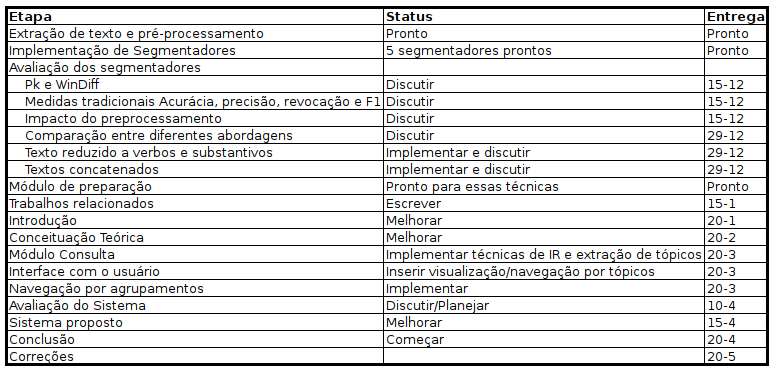
\includegraphics[width=\textwidth]{crono.png}
	\label{fig:exemplosegmentacaozoom}

  \end{figure}






%
%\begin{description}
%
%	\item[1 - Módulo de Preparação e Manutenção:] Esse módulo do sistema deve receber uma coleção de documentos realizar a etapa de  preprocessamento que entrega cada texto separado em segmentos. Em seguida cada segmento deve receber rótulos os quais irão compor uma estrutura de dados, a qual será utilizada para consulta.
%%	
%	Também terá a responsabilidade de incorporar novos documentos à estrutura de dados, bem como recalibrar os algoritmos.
%	
%		
%	\item[2 - Módulo de Busca:] O sistema deve permitir ao usuário buscar por menções sobre um assunto, bem como encontrar e navegar pelos documentos. Para isso, o sistema necessita de um módulo de busca por assuntos. Nesse módulo, a \textit{string} de entrada do usuário deve ser tratada e comparada à base de dados dos documentos já processados, para então exibir ao usuário os trechos correspondentes à busca.
%
%	
%	
%	\item[3 - Avaliação do Sistema:] O sistema final deve ser avaliado junto a usuários a fim de avaliar a eficiência do sistema em suas respostas bem como funcionalidades do ponto de vista de experiência do usuário. 
%%
%Para isso, novamente será necessário a ajuda de voluntários que se enquadram no perfil de usuários alvo.
%%	
%	Após avaliação, uma eventual otimização das técnicas deve ser considerada para o aprimoramento das ferramentas.
%	
%	
%	\item[4 - Conclusão da Dissertação:] Redigir o texto da dissertação.
%	
%		
%
%\end{description}


%
% \begin{center}
%     \begin{longtable}{|c|c|c|c|c|c|c|c|c|c|c|c|}
%     \caption{Cronograma das atividades}\label{table:cronograma}\\ \hline
%   
%     Atividades & 
%     Agosto     & 
%     Setembro   & 
%     Outubro    & 
%     Novembro   & 
%     Dezembro   &
%     Janeiro    
%     \\ \hline
% 	
%%         A   S   O   N   D   J  	
%     1  & X & X &   &   &   &   \\ \hline
%     2  &   & X & X & X &   &   \\ \hline
%     3  &   &   &   & X & X &   \\ \hline
%     4  &   &   & X & X & X &   \\ \hline
%
%     \end{longtable}
% \end{center}





%	\item[2 - Módulo de Classificação:] Os segmentos extraídos devem ser automaticamente classificados em, por exemplo, \emph{decisão}, \emph{menção}, \emph{irrelevante}. %, a fim de 
%Para isso, a partir de um conjunto de treinamento, será construído um modelo de classificação o qual irá induzir uma função capaz de identificar se um documento pertence a determinada classe.

%	\item[Otimizações do Sistema:] 


%	À medida que novos documentos são inseridos ao sistema, faz-se necessário rotinas para a inserção desses na base dados, bem como recalibragem dos algoritmos. % ver com rafael se o extrator de tópicos carece de ser rodado novamente na base toda.
% ver com o rafael se as palavras que extrator fornece podem ser chamadas de rótulos.
	


%Para isso, um classificador deve ser treinado com os rótulos obtidos com os participantes das reuniões.



%\begin{description}

	
%	\item[Implementação do sistema:] O módulo de extração de tópicos necessita de otimizações quanto quanta a eficiência. O módulo de pesquisa necessita de uma interface com o usuário. O sistema após concluído deve ser avaliado comparando-o com a rotulação manual fornecida pelos voluntários.
	
%	\item[Avaliação:] 
	

%\end{description}



%Tarefas como a segmentação textual e a extração de tópicos demandam estudo mais aprofundado. A implementação de ferramentas para teste e rotulação exigiram tempo exta para seu desenvolvimento. 


%	\item[1 - Revisão bibliográfica:] A literatura referente a extração de tópicos deve ser estudada com maior profundidade a fim de aperfeiçoar a dissertação e obter referências de técnicas que compõem o estado-da-arte nesse assunto. %--> outras alternativas surgiram segmentadores que extraem tópicos


%	\item[3 - Conclusão da dissertação:] Os resultados obtidos com a versão final do sistema devem ser incorporados ao texto da dissertação bem como uma revisão da literatura.





